\chapter{Core}
	\section{Organisation des packages}

		L'organisation des packages est la suivante :

		\begin{figure}[H]
			\centering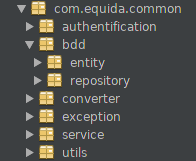
\includegraphics[width=0.33\textwidth, keepaspectratio]{res/core-package.png}
			\caption{Packages de Core}
		\end{figure}

		\begin{description}
			\item[authentification :]{Contient toutes le classes relatives à l'authentification}
			\item[bdd :]{Contient toutes les classes relatives à la \bdd{}}

			\begin{description}
				\item[entity :]{Contient toutes les classes Métiers}
				\item[repository :]{Contient toutes les classes qui héritent de CrudRepository}
			\end{description}

			\item[converter :]{Contient toutes les classes qui héritent de AttributeConverter}
			\item[exception :]{Contient toutes les Exceptions}
			\item[service :]{Contient toutes les classes Services}
			\item[utils :]{Contient quelques classes utiles (Sha256PasswordEncoder, DateUtils, ...)}
		\end{description}

	\section{Exemple d'Entity}

		Une entité est la correspondance de la BDD dans une classe Java. \newline
		Ainsi, on annote la classe de la mention @Entity et on précise avec @Table le nom de la table.

		\newpage
		Ensuite, on crée les variables annotées avec @Colum correspondant aux differents champs de la table. \newline
		Pour l'id on précisera, en plus du fait qu'il s'agit d'un id avec @Id, qu'il est auto-généré avec @GeneratedValue.\newline
		Pour les relations ManyToOne, OneToMany, ect. On utilisera @OneToMany (ou autre en fonction de la relation)\newline
		Pour finir, on inplémente le(s) constructeur(s) ainsi que le(s) getter et setter.

		\begin{figure}[H]
			\centering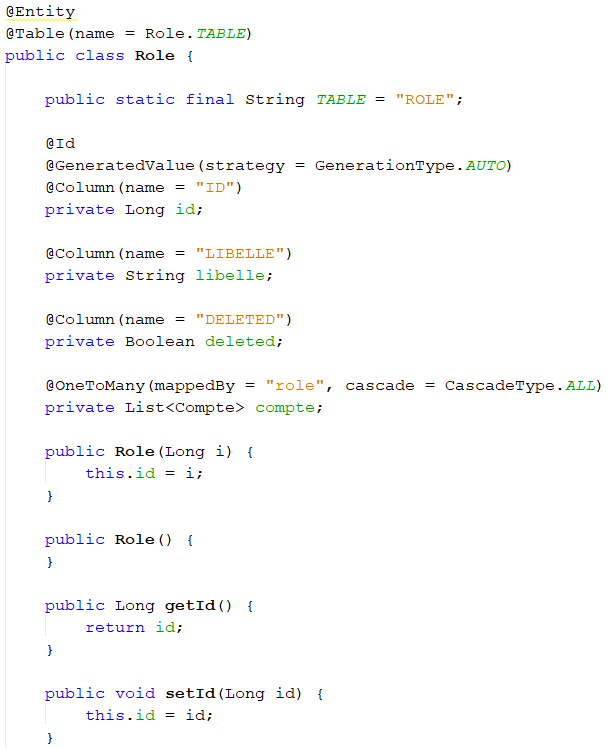
\includegraphics[width=0.80\textwidth, keepaspectratio]{res/entity.png}
			\caption{Exemple extrait du code de l'entity Role}
		\end{figure}

	\newpage
	\section{Exemple de Repository}

		Le repository se charge des requêtes à la BDD pour l’entité correspondante.	Ainsi, on annote la classe de la mention @Repository. \newline

		\noindent
		Ensuite, on implémente les requêtes sql souhaitées dans les @Query. Ces requêtes seront appelées dans le service de l'entité.

		\begin{figure}[H]
			\centering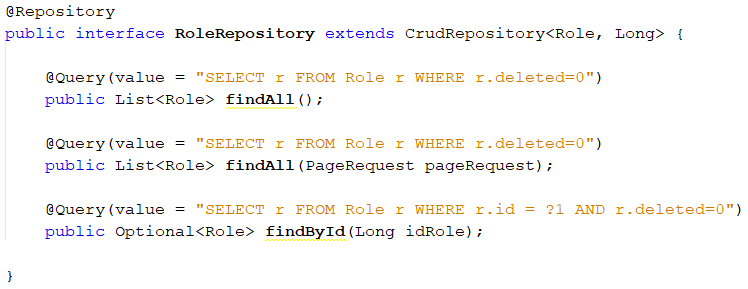
\includegraphics[width=0.80\textwidth, keepaspectratio]{res/repository.png}
			\caption{Exemple extrait du code du repository Role}
		\end{figure}

	\section{Exemple de Service}

		Le service sert d’interface entre le repository et le controller de l'entité qui permettra, en plus, une meilleure gestion des contrôles et des erreurs.\newline
		Ainsi, on annote la classe de la mention @Service. \newline

		\noindent
		Ensuite on déclare le repository concerné, et on implémente les méthodes du service. Elles retourneront les valeurs des méthodes du repository.

		\begin{figure}[H]
			\centering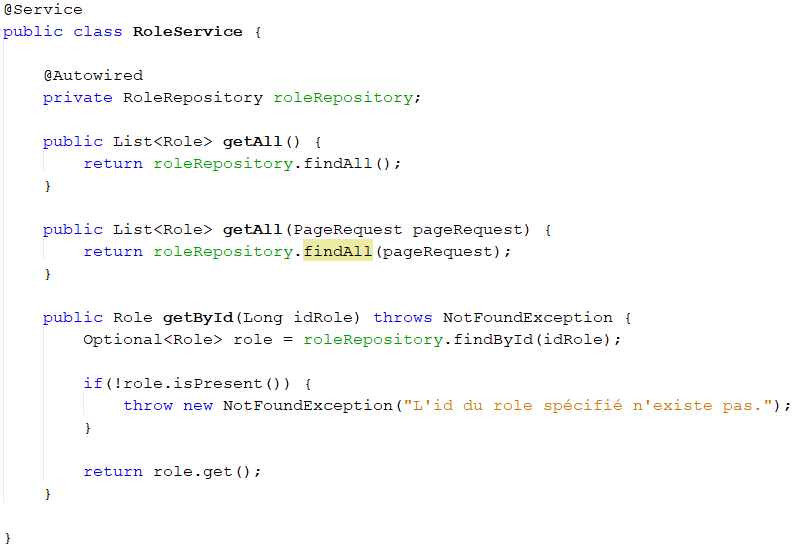
\includegraphics[width=0.80\textwidth, keepaspectratio]{res/service.png}
			\caption{Exemple extrait du code du service Role}
		\end{figure}

	\newpage
	\section{Exemple d'exception (NotFoundException)}
		Le module Core permet de fournir certaines exceptions. Actuellement elles sont au nombre de 4.

		\begin{figure}[H]
			\centering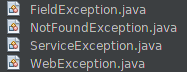
\includegraphics[width=0.30\textwidth, keepaspectratio]{res/exceptions.png}
			\caption{Les différentes exceptions}
		\end{figure}

		\begin{description}
			\item[FieldException :]{Permet de signaler une erreur sur un champs d'un formulaire alors que l'information saisie est valide d'un point de vue HTML. Par exemple, si un SIRE saisi n'existe pas dans la \bdd{} ou, autre exemple, un login saisi existe déjà en \bdd{}, cette erreur est déclenchée.}
			\item[NotFoundException :]{Permet, notamment, de signaler que l'enregistrement demandé n'existe pas dans la \bdd{} ou bien que l'utilisateur n'est pas autorisé à le voir, comme c'est le cas avec un cheval qui appartient à un autre client, par exemple.}
			\item[ServiceException :]{Permet de signaler une erreur dans le comportement du Service. Elles sont surtout utilisées pour signaler qu'un champs requis vaut null.}
			\item[WebException :]{Permet d'encapsuler une exception pour ne pas gêner l'affichage utilisateur. Lors d'un ServiceException, par exemple, l'envoie d'un WebException permet d'afficher une page d'erreur personnalisée.}
		\end{description}

		Le code des exceptions est plutôt simple et court. Voici, par exemple, le code pour NotFoundException.

		\begin{figure}[H]
			\centering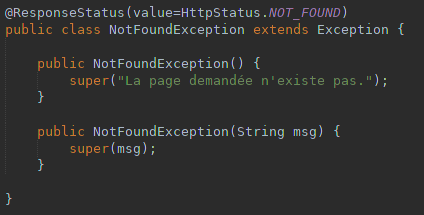
\includegraphics[width=0.75\textwidth, keepaspectratio]{res/NotFoundException.png}
			\caption{Code de NotFoundException}
		\end{figure}

		On définit un simple message d'erreur et on change le code de réponse HTTP, grace à l'annotation @ResponseStatus, afin qu'il renvoie le code 404 et affiche la page adéquate.

	\newpage
	\section{Authentification}
		\label{sec:core_authentification}

		Ce package permet de gérer les différentes classes communes à l'authentification de l'utilisateur pour les modules Rest et WebApp. On y retrouve 2 classes :

		\begin{description}
		   \item[AuthentificationService :]{Cette classe implémente l'interface \textit{UserDetailsService}. Elle permet, pour un login donné, d'aller récupérer l'utilisateur correspondant dans la \bdd{} et retourne un objet de type \textit{AuthentificatedUser}.}
		   \item[AuthentificatedUser :]{Représente l'utilisateur actuellement connecté. Cette classe implémente l'interface \textit{UserDetails}. On y retient notamment la classe Compte qui est la classe métier de la table COMPTE dans la \bdd{}. Grace à cet attribut, on pourra facilement obtenir les informations sur l'utilisateur connecté, par le biais de la méthode \textit{Utilisateur getUtilisteur()}.}
	   \end{description}

	   L'authentification sera alors gérée de manière différente selon le module. Dans le cas du module WebApp, il s'agira d'une connexion par le biais d'une page web tandis que pour l'api Rest on utilisera \href{https://fr.wikipedia.org/wiki/Authentification\_HTTP#M%C3%A9thode\_%C2%AB\_Basic\_%C2%BB}{Basic Authentification}.

	\section{Utils}

		\subsection{DateUtils}

			Cette classe permet de gérer certaines fonctionnalités au niveau des dates. On peut par exemple citer la méthode \textit{boolean isBetween(Date, Date, Date)} qui permet de savoir si la dernière Date est comprise entre les 2 premières. Cette classe permet également d'afficher une date fournie en paramètre au format "jour/mois/année" grâce à la méhode \textit{String format(Date)}.

		\subsection{Sha256PasswordEncoder}
			\label{subsec:Sha256PasswordEncoder}

			Cette classe permet de gérer le hachage des mots de passe. Elle implémente l'interface \textit{PasswordEncoder}. qui fournit une méthode publique \textit{String encode(CharSequence)}. Cette méthode retourne en String le hachage, en sha256 dans notre cas, de la chaine de caractères fournie en paramètre. Cette classe est transmises à Spring Security afin de vérifier les informations saisies par l'utilisateur lors d'une connexion. Elle est également utilisée manuellement lors de l'enregistrement d'un nouveau client.
